%%%%%%%%%%%%%%%%%%%%%%%%%%%%%%%%%%%%%%%%%
% FRI Data Science_report LaTeX Template
% Version 1.0 (28/1/2020)
% 
% Jure Demšar (jure.demsar@fri.uni-lj.si)
%
% Based on MicromouseSymp article template by:
% Mathias Legrand (legrand.mathias@gmail.com) 
% With extensive modifications by:
% Antonio Valente (antonio.luis.valente@gmail.com)
%
% License:
% CC BY-NC-SA 3.0 (http://creativecommons.org/licenses/by-nc-sa/3.0/)
%
%%%%%%%%%%%%%%%%%%%%%%%%%%%%%%%%%%%%%%%%%


%----------------------------------------------------------------------------------------
%	PACKAGES AND OTHER DOCUMENT CONFIGURATIONS
%----------------------------------------------------------------------------------------
\documentclass[fleqn,moreauthors,10pt]{ds_report}
\usepackage[english]{babel}
\usepackage{listings}
\usepackage{natbib}
\usepackage{acro}
\graphicspath{{fig/}}
\usepackage{xcolor}
\usepackage[most]{tcolorbox}
\usepackage{subcaption}
\usepackage{cleveref}
\usepackage{changepage}

\newcommand{\red}[1]{\textcolor{red}{#1}}
\newcommand{\green}[1]{\textcolor{green}{#1}}

\lstset{
frame=none,
extendedchars=false,
inputencoding=utf8/latin1
}

%----------------------------------------------------------------------------------------
%	ARTICLE INFORMATION
%----------------------------------------------------------------------------------------

% Header
\JournalInfo{FRI Natural language processing course 2025}

% Interim or final report
\Archive{Project report} 
%\Archive{Final report} 

% Article title
\PaperTitle{Conversational Agent with Retrieval-Augmented Generation} 

% Authors (student competitors) and their info
\Authors{Matej Belšak, Gorazd Gorup, Luka Bajić}

% Advisors
\affiliation{\textit{Advisors: Aleš Žagar}}

% Keywords
\Keywords{Conversational agent, Retrieval-Augmented Generation}
\newcommand{\keywordname}{Keywords}


% Abbreviations
\DeclareAcronym{llm}{
	short=LLM,
	long=Large Language Model
}

\DeclareAcronym{rag}{
	short=RAG,
	long=Retrieval Augmented Generation
}

\DeclareAcronym{nlp}{
	short=NLP,
	long=Natural Language Processing
}

\DeclareAcronym{tmdb}{
	short=TMDB,
	long=The Movie Database
}

\DeclareAcronym{fifo}{
	short=FIFO,
	long=First-In-First-Out
}

\newcommand{\etal}{\textit{et al}., }
\newcommand{\ie}{\textit{i}.\textit{e}., }
\newcommand{\eg}{\textit{e}.\textit{g}.\ }


%----------------------------------------------------------------------------------------
%	ABSTRACT
%----------------------------------------------------------------------------------------

\Abstract{
Develop a conversational agent that enhances the quality and accuracy of its responses by dynamically retrieving and integrating relevant external documents from the web. Unlike traditional chatbots that rely solely on pre-trained knowledge, this system will perform real-time information retrieval, ensuring up-to-date answers. Potential applications include customer support, academic research assistance and general knowledge queries. The project will involve natural language processing, web scraping, and retrieval-augmented generation techniques to optimize answer quality.
}

%----------------------------------------------------------------------------------------

\begin{document}

% Makes all text pages the same height
\flushbottom 

% Print the title and abstract box
\maketitle 

% Removes page numbering from the first page
\thispagestyle{empty} 

%----------------------------------------------------------------------------------------
%	ARTICLE CONTENTS
%----------------------------------------------------------------------------------------

\section*{Introduction}
	
While \acp{llm} have evolved considerably and now produce convincing replies, they have inherent limitations. They rely on training data consisting of documents from the past and may not possess knowledge of current events and developments. Due to differences and properties of training datasets, they may not contain specific domain knowledge, failing to answer certain prompts or outright hallucinating. The latter could prove especially disastrous in dedicated chatbots, for example for legal guidance or health care~\cite{thirunavukarasu2023large}.

One possibility would be to retrain the chat model in intervals to try to keep it up to date, but that would still produce periods where the information is missing from the \ac{llm} or is outdated. This approach, while completelly time and energy inefficient, would also not guard against hallucinations. To solve these issues, \ac{rag} is used to provide the missing knowledge to the \ac{llm}. \ac{rag} employs different techniques to retrieve information from external sources based on user’s prompt and through prompt augmentation feed the \ac{llm} sufficient information to provide informative and factually correct answer. In the survey by Gao~\etal~\cite{survey}, multiple approaches to \ac{rag} are presented, highlighting three architectures: naive \ac{rag}, which analyzes the user’s prompt, retrieves the required information and appends it, letting the \ac{llm} do the rest; advanced \ac{rag}, which employs pre-retrieval and post-retrieval modifications to the prompt to make it more suitable for information retrieval and subsequent interpretation by \ac{llm}; lastly, modular \ac{rag} combines multiple approaches, using iterative prompt enhancement, ranking, fusion, etc.

For document summarization, \acp{llm}, statistical models, graph-based models and other approaches are used to extract the most important information from text. Zhang~\etal~\cite{summarization} present multiple solutions, noting that \acp{llm}, while consuming more resources, tend to be more coherent and precise in their summarization if trained correctly.

In this paper, we focus on \ac{rag} methods and their use in chatbots. To that end, we design a conversational agent operating on knowledge about different art and media. Specifically, the agent is to suggest and converse about films and other related media based on the user’s prompts and preferences. Our contributions are:

\begin{itemize}
	\item Implementation of a conversational agent using two different pretrained models: DeepSeek-R1~\cite{deepseek3} and Qwen 3~\cite{qwen3}.
	\item Implementation of two \ac{rag} techniques, a primitive and advanced one, with capabilities of retrieving data from various film-related databases and web sources.
	\item Evaluation of conversational agents with respect to the model used and the \ac{rag} technique. Agents are evaluated against the baseline \ac{rag}-less chatbots. Human and \ac{llm} judges are used to score responses, and different metrics are analyzed.
\end{itemize}

%------------------------------------------------

\section*{Methods}

We designed two \ac{rag} pipelines, as presented in~\cref{fig:pipeline}. The naive RAG pipeline used \ac{nlp} methods to extract the important feature information from prompt via lemmatization, stop-word removal, and entity detection. Prompt information was used to determine movie titles and names of people to query for in our selected databases. That information was then appended to the prompt and fed into an \ac{llm}.

A more advanced version of our \ac{rag} system utilized various components, but we ultimately chose to employ function-calling functionality that is present in some \acp{llm}. Based on the prompt, the \ac{llm} decides on the most appropriate information retrieval function to call and informs the \ac{rag} system, which then retrieves that information. The information is then inserted into the prompt, which is fed into the \ac{llm}.

\begin{figure*}
	\centering
	\begin{subfigure}{0.4\textwidth}
		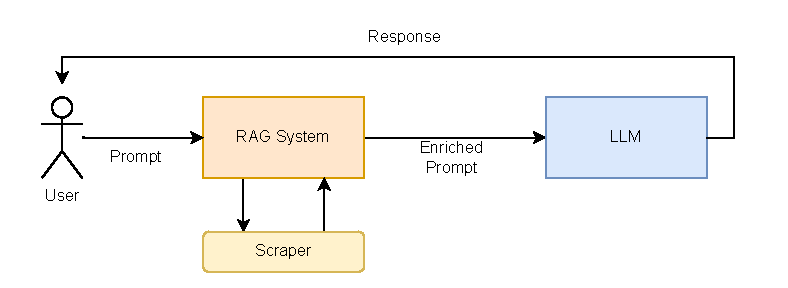
\includegraphics[width=\textwidth]{./figures/simple_rag.pdf}
		\caption{A naive \ac{rag} system.}
	\end{subfigure}
	\hspace{20pt}
	\begin{subfigure}{0.4\textwidth}
		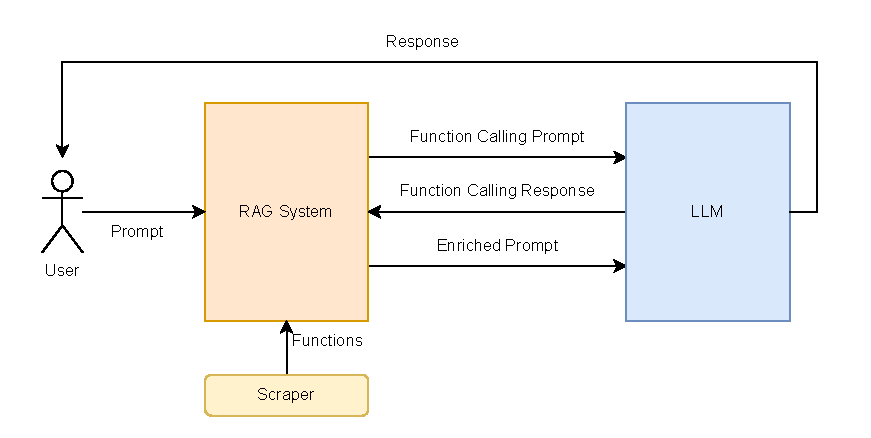
\includegraphics[width=\linewidth]{./figures/advanced_rag.pdf}
		\caption{An advanced \ac{rag} system.}
	\end{subfigure}
	\caption{Our proposed \ac{rag} pipelines for evaluation. The naive \ac{rag} variant preprocesses the prompt, extracts meaningful information from it, retrieves the data based on that, and enhances the prompt with that raw data. The advanced variant employs \ac{llm} function-calling capabilities to decide what data to scrape and enhances the prompt only with necessary data.}
	\label{fig:pipeline}
\end{figure*}

\subsubsection*{Function Calling}

In some cases, we leveraged the function calling capabilities of our models. While DeepSeek hints at possibility of using this feature~\cite{deepseekFunctionCalling}, their proposed prompt templates do not support it. We instead turned to Qwen's function calling capabilities, which proved to be sufficient.

In function calling, the model is presented with the user prompt and structured information about programmatic functions it may call to fullfil the user's request. The \ac{llm} is tought to return a similarly structured set of instructions on which functions to call, and with what parameters.

\subsection*{Information Retrieval}

To provide a sufficient level of information related to movies and similar media, we selected the following sources:

\begin{itemize}
	\item \textbf{\ac{tmdb}.} This is an open database of movies, TV-shows, and people associated with them. They provide a free-to-use API for various types of requests -- release dates, cast, crew, similar films ...
	\item \textbf{Letterboxd.} This is a movie-themed social network to log watched films, provide reviews, and engage in movie-related discussions. We chose to include it to give the model a better understanding of how people percieve certain media.
	\item \textbf{JustWatch.} This website tracks the availability of media on digital and streaming platforms.
	\item \textbf{Wikipedia.} We used it to retrieve information such as film plots, summaries, etc.
\end{itemize}

In our naive \ac{rag} implementation, we retrieved data from all four sources. This would amount to over 250,000 characters of context.

For our advanced version, we prepared nine custom scraping functions that would equip the model with essential information about movie titles and film-related people. These functions had to be specifically annotated and various versions of descriptions were used to elicit a proper function-calling response from the model.

\subsection*{\ac{rag}}

For the naive \ac{rag} system, we first analyzed the user prompt and gathered all relevant entities, consisting of film titles and names of people. We used a Roberta-like \texttt{spacy} model~\footnote{https://huggingface.co/spacy/en\_core\_web\_sm}. We performed unfiltered knowledge injection, gathering all relevant documents based on prompt entities, structured them in JSON format, and passed them allong with user query to the \ac{llm}.

For advanced \ac{rag} system, we tried several versions before basing it on function calling. Our earlier attempts performed the entity extraction from prompt, retrieval of documents from all sources based on those entities, and content curation based on statistical methods and user prompt. For example, we treated all sentences in the retrieved data as documents, performing TF-IDF sorting and using only top $N$ most relevant sentences. Unfortunatelly, results of these extractions accounted only for literal appearance of words from the prompt in documents, instead of accounting for larger context, synonyms, etc.

To address these shortcomings, we turned to function calling, letting the \ac{llm} decide what information to retrieve. In the system prompt, we also appended additional information about current date for better context formulation.

With function calling, we also had to thoroughly describe all available functions to the \ac{llm}, which proved challenging, as the model sometimes failed to infer the correct connection between the user's input and the function descriptions.

\subsection*{Prompt formulation}

We structured our prompts to consist of three roles: system, user, and assistant. We put system prompt first, followed by the user prompt, and finally by assistant tag to signal the \ac{llm} to generate the answer, not to continue the user prompt.

Our system prompt was:

\begin{figure}[h!]
	\begin{tcolorbox}
		You are an AI chatbot, assisting user with anything related to movies. [Today's date is \verb|{date}|.] You may only use information provided to you inside the \verb|<data>| tags.
	\end{tcolorbox}
	\caption{Out prompt for \ac{rag} usage. The text in square brackets was only used in advanced \ac{rag}, and the text in braces represents variables.}
\end{figure}

Our user prompt first presented the user's initial query, followed by the retrieved information enclosed in \verb|<data>| tags.

A key challenge during this stage was ensuring that the LLM relied solely on the provided information and avoided generating unsupported content. Despite clear instructions, it was often difficult to prevent the model from hallucinating or making assumptions beyond the data enclosed in the <data> tags.

\subsection*{Memory and chat}

To extend a question answering model into a conversational chatbot, we kept the information retrieval pipeline unchanged and implemented a simple answer caching mechanism to preserve conversational context. Specifically, we stored the last $n$ user queries and chatbot responses using the \ac{fifo} method and included them in the prompt provided to the \ac{llm}. Due to input token limitations, the value of $n$ had to remain relatively small in our experiments to ensure the model could process the full prompt effectively. Otherwise, there was a risk of token truncation and generation errors.

\subsection*{Evaluation methodology}

Since we are working with relatively open-ended questions, there is a lack of objective ground truth to evaluate against. Therefore, we construct a set of 50 domain-relevant questions and use manually checked answers from the commercial ChatGPT model as ground truth for metric computations. To avoid overfitting a model to a specific set of expected outputs, we included multiple types of questions into our test set, including yes/no questions, fact checking, list retrieval and summarization. All queries are zero-shot.


\subsubsection*{LLM-based evaluation}

Standard evaluation metrics such as BLEU and ROUGE are ill-adjusted to our test set, because they penalize diverse answers, which could still be correct in the context of open-ended questions. To bypass this limitation, we employ the DeepEval framework \cite{deepeval} in order to obtain more relevant metrics based on context, query and response:

\begin{itemize}
	\item \textbf{Correctness}: Measures how accurate the response is compared to the ground truth.

	\item \textbf{Clarity}: Evaluates how clear and understandable the response is for the user. (we do not expect to improve this metric with \ac{rag}, we only utilize it to ensure that our modifications do not degrade the original model's inherent capabilities),
	
	\item \textbf{Answer Relevancy}: Assesses how well the response addresses the user's input and stays on topic.
	
	\item \textbf{Faithfulness}: Measures whether the response is factually consistent with the provided context, without introducing unsupported claims.
	
	\item \textbf{Contextual Precision}: Evaluates whether relevant pieces of context are ranked higher than irrelevant ones for the given user's input.
	
	\item \textbf{Contextual Recall}: Measures how well the retrieved context covers the information needed to produce the ground truth response.
	
	\item \textbf{Contextual Relevancy}: Assesses the overall relevance and usefulness of the retrieved context for answering the user's input.

\end{itemize} 

The correctness, clarity, and answer relevancy show the \ac{llm}'s focus on the retrieved information with respect to the ground truth and the user's query. Faithfulness measures the \ac{llm}'s capability to properly use the retrieved information. Precision, recall, and contextual relevancy all present the performance of the retrieval system. The models were judged on scale from 0 to 1. 

\section*{Results}

\begin{table*}[t]
%\centering
\resizebox{1.0 \linewidth}{!}{\begin{tabular}{| r | c c c c c c c |}
\hline
model & correctness & clarity & answer relevancy & faithfulness & contextual precision & contextual recall & contextual relevancy \\ \hline
deepseek-baseline  & 0.1280 & 0.7780 & 0.7657 & \textemdash & \textemdash & \textemdash & \textemdash \\
deepseek-naive  & 0.1720 & 0.7800 & 0.6846 & 0.9310 & 0.1600 & 0.5097 & 0.4238   \\
deepseek-advanced  & 0.2440 & 0.6920 & 0.8055 & \textbf{0.9397} & \textbf{1.0000} & \textbf{1.0000} & \textbf{0.5580}  \\
qwen-baseline  & 0.2950 & \textbf{0.8950} & 0.7283 & \textemdash & \textemdash & \textemdash & \textemdash  \\
qwen-naive & 0.2780 & 0.8425 & \textbf{0.8510} & 0.8530 & 0.9500 & 0.8950 & 0.3370  \\
qwen-advanced & \textbf{0.4400} & 0.8200 & 0.7411 & 0.9280 & 0.2000 & 0.4000 & 0.1774 \\
\hline
\end{tabular}}
\caption{Performance comparison as evaluated by a 14B-parameter Qwen model with DeepEval framework.}
\label{tab:llm_metrics}
\end{table*}

\begin{table*}[t]
%\centering
\resizebox{1.0 \linewidth}{!}{\begin{tabular}{| r | c c c c c c c |}
\hline
model & correctness & clarity & answer relevancy & faithfulness & contextual precision & contextual recall & contextual relevancy \\ \hline
deepseek-baseline  & 0.3185 & 0.7492 & 0.6172 & \textemdash & \textemdash & \textemdash & \textemdash \\
deepseek-naive  & 0.3341 & 0.8144 & 0.7207 & 0.7561 & 0.3400 & 0.3201 & 0.4362   \\
deepseek-advanced & 0.3341 & 0.7841 & 0.8097 & 0.9301 & \textbf{1.0000} & 0.6094 & 0.5681   \\
qwen-baseline  & 0.4521 & 0.8102 & \textbf{0.8794} & \textemdash & \textemdash & \textemdash & \text{\textemdash}  \\
qwen-naive  & 0.4512 & 0.7799 & 0.8001 & 0.8323 & 0.3400 & 0.2644 & 0.5164  \\
qwen-advanced & \textbf{0.5234} & \textbf{0.8338} & 0.6804 & \textbf{0.9794} & \textbf{1.0000} & \textbf{0.6110} & \textbf{0.6836}   \\
\hline
\end{tabular}}
\caption{Performance comparison as evaluated by GPT-4.1-mini model with DeepEval framework.}
\label{tab:gpt}
\end{table*}


Since we were limited by hardware capabilities during our research, we focused on models with quantized or distilled variants. We ultimatelly decided on a Qwen3 \cite{qwen3}~\footnote{https://huggingface.co/Qwen/Qwen3-8B} model as our non-reasoning \ac{llm}, and a distilled Llama variant of DeepSeek R1 \cite{deepseek3}~\footnote{https://huggingface.co/deepseek-ai/DeepSeek-R1} as our reasoning \ac{llm}. Both models were loaded from HuggingFace and were run through the \texttt{transformers} API.

Both models were 8-billion-parameters versions. We chose DeepSeek as it is a novel set of models with positive benchmarking results~\cite{deepseek3}. For each of these, we run experiments on three different sets of parameters:
\begin{itemize}
	\item without \ac{rag} - out-of-the-box model with no modifications (baseline)
	\item with naive \ac{rag} - all documents are retrieved and appended to the context with no consideration for token limitation (data is truncated)
	\item advanced \ac{rag} - documents are selectively retrieved and processed before being appended to the context
\end{itemize}

Results obtained with Qwen3-14B model are shown in Table \ref{tab:llm_metrics}. Metrics related to context are not available for baseline models, because their context is an empty set. Models with advanced \ac{rag} can choose not to retrieve documents, depending on the user query, so the context-related metrics are only computed when at least one document was retrieved.

Because the model used for evaluation is not drastically larger than the model used for response generation, it is sensible to repeat the same experiments with an even larger LLM to obtain more reliable results. We opted for GPT-4.1-mini. Results are shown in Table \ref{tab:gpt}. Due to computational complexity, we compute the metrics on first 25 questions in the test set and report the average values. 

\subsection*{Conversational chatbot}
In advanced \ac{rag}, we observed that the memory mechanism prevented the chatbot from being confused about queries referencing previous ones, managing to remember crucial data for function calling. Sometimes, the \ac{llm} even decided against retrieving information in queries where it otherwise would, because previous questions and answers provided enough information or context to formulate a sufficient response.

Examples of Qwen chatbot results are shown in Appendix \ref{qwenconvo}.


\section*{Discussion}

% TODO: Abstract

% TODO: Prompt formulating: Difficult to get LLM to not make stuff up and only use provided information.

% TODO: Function calling: difficulties with describing the functions in a way that would make the LLM call that function in the desired context. (CHECK)

% TODO: Letterboxd reviews provided a mixed-quality source, (LATER)

%------------------------------------------------

%We conclude that it is possible to improve the responses of 8B-parameter LLMs, such as Qwen and DeepSeek on queries from a specific domain by employing on-the-fly information retrieval via web scraping. 

%Superior performance is achieved by constructing document retrieval functions in such a way that an LLM can be used not only to generate a response, but also to determine which documents are relevant based on the user query. 

%A question answering model with \ac{rag} can be extended into a chatbot by implementing a memory mechanism, which stores a buffer of previous questions, which allows the model to keep track of recent conversation.

As seen in Table \ref{tab:llm_metrics}, Qwen judge scores DeepSeek with advanced RAG quite high on the information retrieval metrics, while prefering Qwen in \ac{llm} answer generation based on ground truth and user prompt. Qwen with advanced RAG is considered to be the most in line with ground truth answers. Interestingly, Qwen judge considers even the best model to perform poorly on more than half the questions in regards to correctness.

Table \ref{tab:gpt} shows that GPT tends to evaluate the results more favorably than Qwen.

Notably, Qwen with advanced RAG system performs best in most metrics. Specifically, it generally generates responses relevant to the user's question. When given context, it follows the provided information most faithfully. It performs somewhat decent when compared to the ground truth, passing over 50\% of the tests.

Our advanced RAG system shows that our retrieved data is mostly aligned with what is expected, although we sometimes present the \ac{llm} with irrelevant information. This can be attributed due to the fact that our retrieval does not perform granular information extraction, instead relying on function-calling model to pick specific (short) documents of information to retrieve.

Baseline Qwen returns more relevant answer, which we could attribute to the fact that it has the most freedom to when answering, not tied to the context which could lead the answer to not directly align with what the query is asking, or cause the \ac{llm} to populate the answer with uncessesary details.

In addition to evaluating RAG methods, we also explored how large a model needs to be to effectively serve as an \ac{llm}-as-judge for smaller models. We compared the performance of Qwen3-14B and GPT-4.1-mini as judges. Based on both metric results and manual inspection of model outputs against ground truth answers, we observed that GPT-4.1-mini was better at fairly and accurately evaluating responses. Qwen3-14B often failed to do so reliably, which is why we place more trust in GPT-based evaluations. Our results also confirm that the advanced RAG approach consistently outperforms the naive one across models. Qwen with advanced RAG performs better than DeepSeek with advanced RAG. DeepSeek's reasoning capabilities may sometimes interfere with faithfully following retrieved context, leading to incorrect assumptions. In contrast, Qwen tends to adhere more closely to the provided input, which may contribute to its stronger performance in this setting.


%----------------------------------------------------------------------------------------
%	REFERENCE LIST
%----------------------------------------------------------------------------------------
\bibliographystyle{unsrt}
\bibliography{report}

\newpage
\begin{appendix}

\section*{Appendix}
\label{append}

\subsection*{Qwen conversation example}

\begin{figure}
\begin{tcolorbox}
User: How many films did Chuck Jones make?

Qwen: Based on the data provided:

	**Total Number of Films:**  
	Chuck Jones directed **over 100 films**, spanning multiple genres and formats.

	\#\#\# Breakdown:
	- **Feature-Length Films**: 
    		- *The Bugs Bunny/Road Runner Movie* (1979)
	    - *The Phantom Tollbooth* (1970)
	    - *The Grinch Stole Christmas!* (1966)

	- **Shorts and Documentaries**:
	    - Approximately **100+ short cartoons**
	        - Many of these are Looney Tunes/Merry Melodies cartoons.
	        - Includes iconic titles such as *What's Opera, Doc?*, *Duck Amuck*, etc.
    
	    - **Documentaries**: Around **dozens**, e.g.,
	    	    - *The Magical World of Chuck Jones*
	        - *Chuck Jones: Memories of Childhood*

	\#\#\# Summary:
	Chuck Jones made approximately \textbf{more than 100 films}, primarily consisting of **\green{animated short cartoons}**, a handful of **\green{feature-length compilations}**, and several **\red{documentaries}**.
\end{tcolorbox}
\caption{Conversation with Qwen}
\label{qwenconvo}
\end{figure}

\begin{tcolorbox}[breakable,float*,width=\textwidth,title=Conversation Example with Advanced Qwen]

\textbf{What is the movie Until Dawn about?}

\begin{adjustwidth}{20pt}{0pt}

\emph{Until Dawn} is a 2025 American \textbf{survival horror film}
directed by \textbf{David F. Sandberg} and written by \textbf{Gary
Dauberman} and \textbf{Blair Butler}. Based on the \textbf{2015 video
game} \emph{Until Dawn} developed by \textbf{Supermassive Games} for
PlayStation, the film adapts the game's eerie atmosphere and gameplay
mechanics---such as the \textbf{time-loop structure} and
\textbf{branching narratives}---into a \textbf{standalone storyline}
within the same fictional universe.

\subsubsection*{Key Details About Until Dawn}

\texttt{[... (omitted due to length)]} \\

\end{adjustwidth}

\textbf{Who directed that movie?}

\begin{adjustwidth}{20pt}{0pt}

The movie \textbf{Until Dawn (2025)} was directed by \textbf{David F.
Sandberg}, a Swedish filmmaker best known for his work on the
\emph{Annabelle} and \emph{Lights Out} franchises. He brought his
signature style of suspenseful horror and atmospheric tension to this
adaptation of the popular video game \emph{Until Dawn}.

\texttt{[... (omitted due to length)]} \\

\end{adjustwidth}

\textbf{Who are the main actors?}

\begin{adjustwidth}{20pt}{0pt}

Here are the \textbf{main cast members} of \emph{Until Dawn (2025)}
along with their roles:

\subsubsection*{Main Cast:}

\begin{tabular}{ l l }
	Actor Name & Role \\
	\textbf{Ella Rubin} & \textbf{Clover Paul} \\
	\textbf{Michael Cimino} & \textbf{Max} \\
	\textbf{Odessa A'zion} & \textbf{Nina Riley} \\
	\textbf{Ji-young Yoo} & \textbf{Megan} \\
	\textbf{Belmont Cameli} & \textbf{Abe} \\
	\textbf{Maia Mitchell} & \textbf{Melanie Paul} \\
	\textbf{Peter Stormare} & \textbf{Dr.~Alan Hill} \\
\end{tabular}

\texttt{[... (omitted due to length)]} 

Would you like information about any particular actor or role from the
film?

\end{adjustwidth}

\end{tcolorbox}
%\caption{Conversation with Qwen}
%\label{qwenconvo}


\end{appendix}


\end{document}